\section{Fazit}

\textsc{Matthias Vongerichten}

Das redaktionelle Konzept beschreibt die vorgesehenen Inhalte je Seite in Kurzform. Au�erdem wird hierbei auch eine Richtlinie zur Aktualisierungsh�ufigkeit je Seite vorgegeben (unterst�tzt SEO). Somit wird erreicht, dass der redaktionelle Verantwortliche eine kompakte Anleitung zur Pflege der Website erh�lt.

Beim Navigationskonzept wurden die wichtigsten Navigationselemente beachtet. Hervorzuheben sind hier die "`Breadcrumb"'-Navigation und die Implementierung von mod\_rewrite (Abbildung ~\ref{abb:htaccess}, Seite ~\pageref{abb:htaccess}).

\textsc{Stefan Waidele}

...

\subsection{Evt. Gesamtfazit}

Die Website erf�llt die gestellten Anforderungen vollst�ndig. So bescheinigt uns woorank.com (SEO-Analyse-Tool), dass z.B. nicht-funktionalen Anforderungen wie die Performance der Site sehr gut erf�llt werden.

\begin{figure}[h]
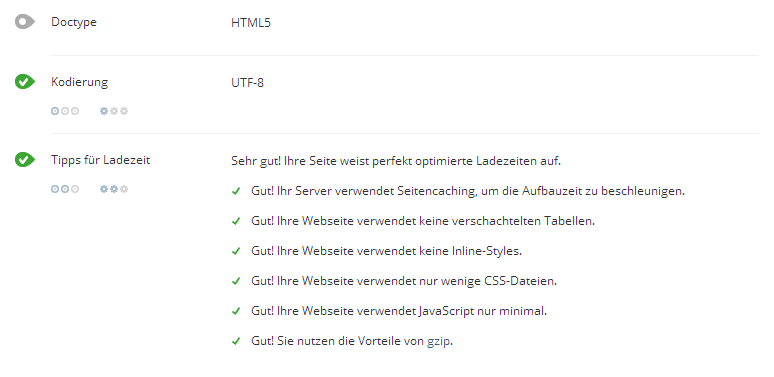
\includegraphics[width=\hsize]{scr_woorank_performance.png}
\caption{Screenshot: Performance}
\label{scr:performance}
\end{figure}
\begin{figure}[h]
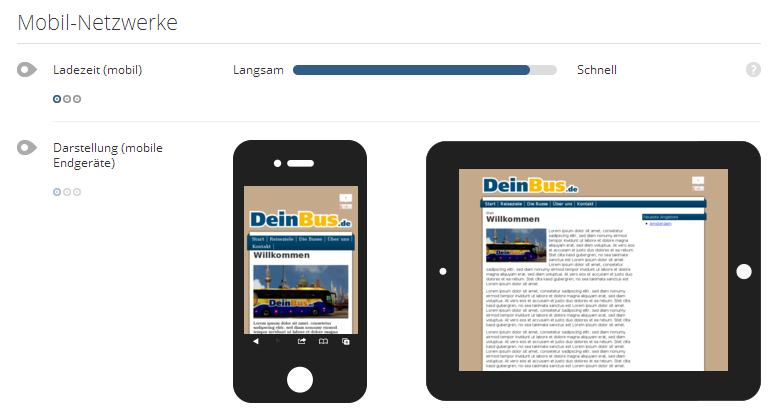
\includegraphics[width=\hsize]{scr_woorank_mobile_performance.png}
\caption{Screenshot: Mobile Ger�te}
\label{scr:mobile}
\end{figure}

%screenshot scr_woorank_performance.png oder scr_woorank_mobile performance.png oder beides

Ein n�chster m�glicher Schritt ist die Verwendung eines Content-Management-Systems (CMS). Dies erm�glicht das einfache Bearbeiten der Seiteninhalte mithilfe eines WYSIWYG-Editors (keine Code-Kenntnisse notwendig) und das Aufrechterhalten eines konsistenten Designs. Die Navigation kann auf mehrere Ebenen und Elemente verteilt werden und aktualisiert sich selbst�ndig. Der Administrationsaufwand wird somit stark reduziert und trotzdem f�llt es erstaunlich leicht die Funktionen der Website durch vorgefertigte Module zu erweitern. So ist es ebenfalls m�glich einen Weblog zu betreiben welcher mit Facebook und anderen Social-Media-Diensten integriert werden kann. Urspr�nglich als Weblog-System zu gro�er Bekanntheit gelangt, kann Wordpress heute als einfaches und komfortables CMS genannt werden. F�r komplexere Anwendungsf�lle eignet sich Drupal oder Typo3.
